\documentclass{article}
\usepackage[utf8]{inputenc}
\usepackage{array}
\usepackage{wrapfig}
\usepackage{multirow}
\usepackage{tabu}
\usepackage{graphicx}

\title{Report}
\author{Tuğrul Tosun}
\date{22.12.20}

\begin{document}

\maketitle
\section{Part 1: K-Nearest Neighbor}
\subsection{K-fold Cross-validation}
\begin{figure}[h!]
  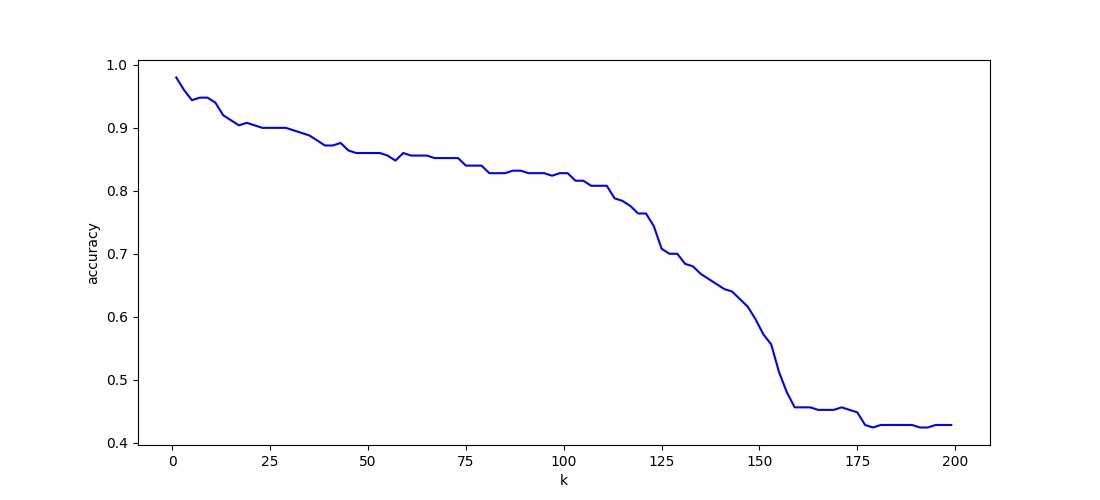
\includegraphics[width=\linewidth]{knn.jpeg}
  \caption{KNN.}
  \label{fig:KNN}
\end{figure}



\subsection{Accuracy drops with very large k values}
As k gets larger majority class of our train set will have impact on our testing results. When k gets larger our knn algorithm will calculate the most occurrence of neighbour for that k so when k get close to our training set size, our data will be classified as the label that occurs more in train set.

\subsection{Accuracy on test set with the best k}
My best k is 1 and accuracy for the test data for k=1 is 0.99(99$\%$). I have also printed these values in my code in last few lines.\\


\maketitle
\section{Part 2: K-means Clustering}
\subsection{Elbow method}
Plot k vs final objective values according to the description in the homework on each clustering data. Decide which k is suitable on each data.

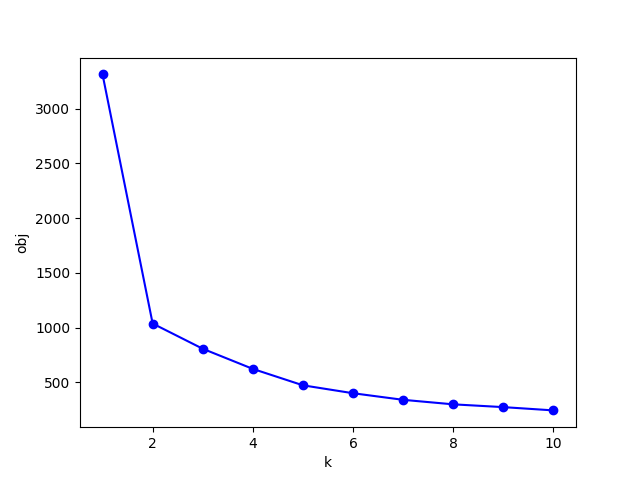
\includegraphics[width=\linewidth]{clustering_images/clustering1obj.png}
\centerline{Clustering 1 data:choosing k=2 for clustering}\\
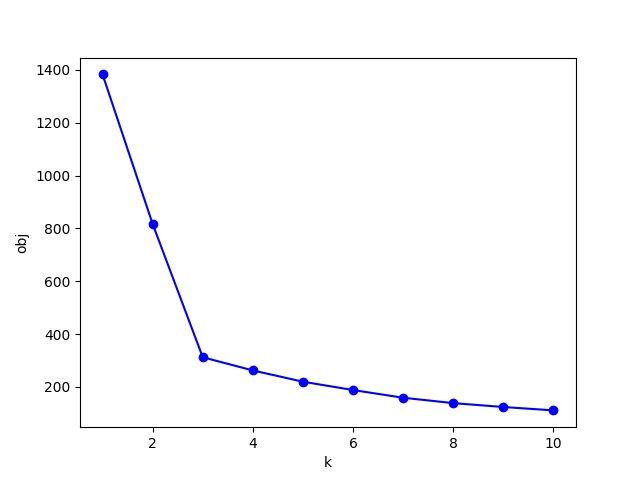
\includegraphics[width=\linewidth]{clustering_images/clustering2obj.png}
\centerline{Clustering 2 data:choosing k=3 for clustering}\\
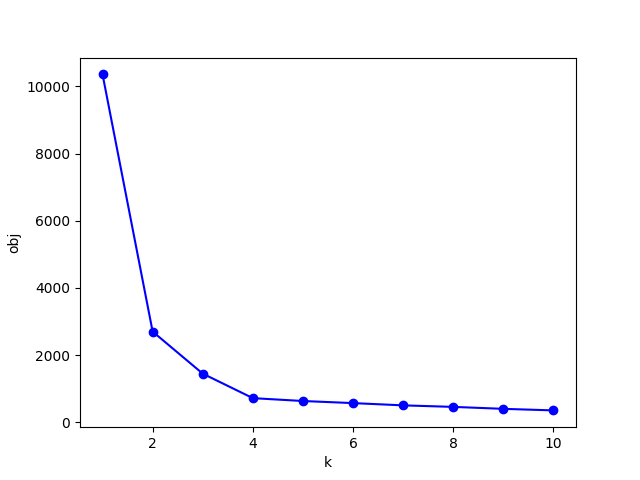
\includegraphics[width=\linewidth]{clustering_images/clustering3obj.png}
\centerline{Clustering 3 data:choosing k=4 for clustering}\\
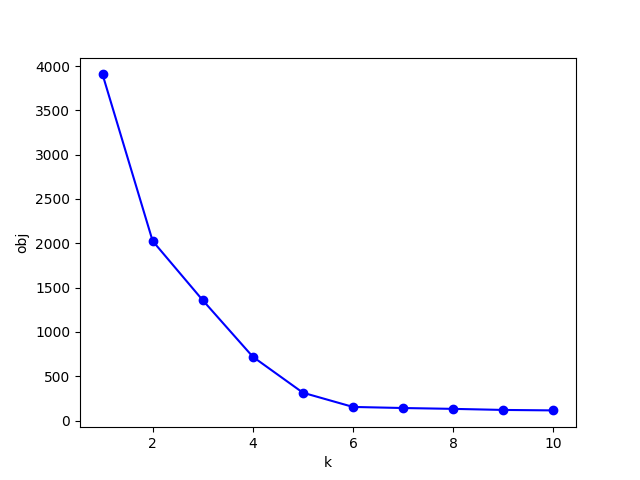
\includegraphics[width=\linewidth]{clustering_images/clustering4obj.png}
\centerline{Clustering 4 data:choosing k=5 for clustering}\\



\subsection{Resultant Clusters}
Plot the final clusters in each data according to the description in the homework.\\

Red stars in figures represent cluster centroids.

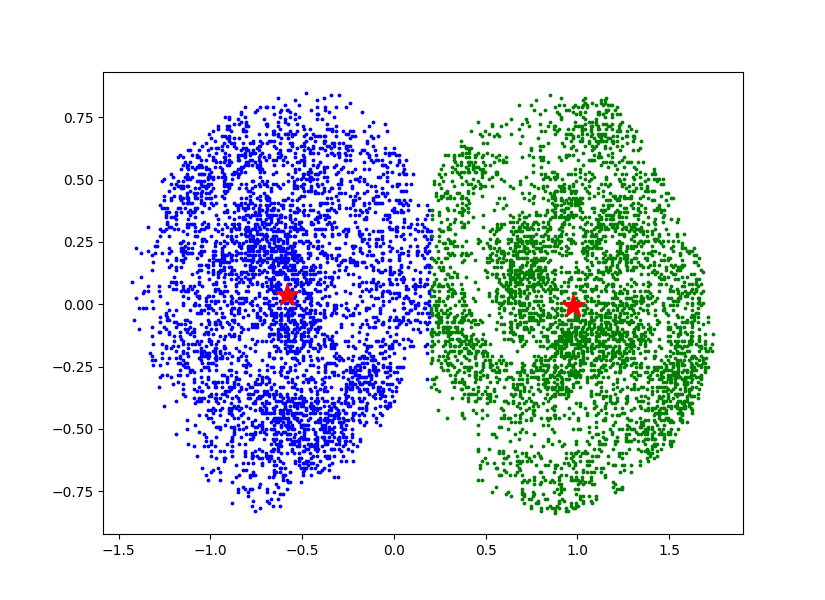
\includegraphics[width=\linewidth]{clustering_images/clustering1kmeans.png}
\centerline{Clustering 1}\\
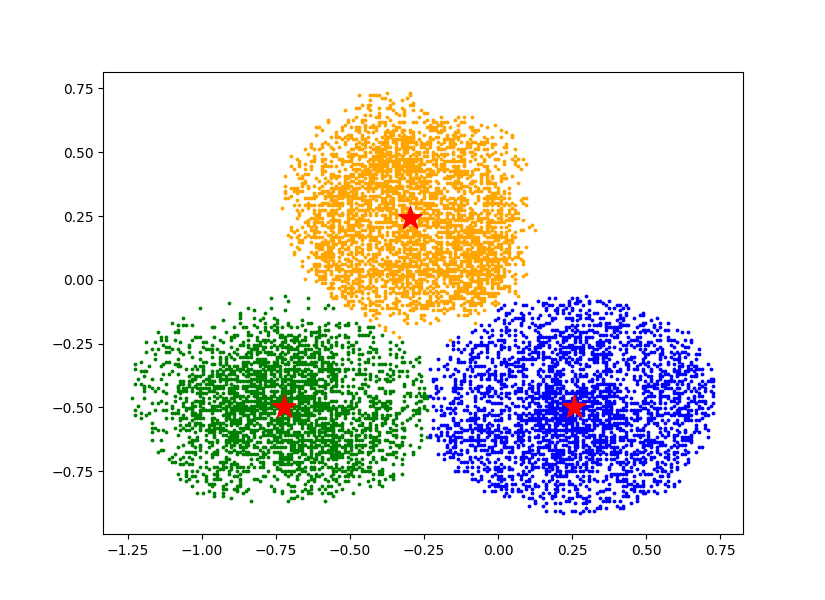
\includegraphics[width=\linewidth]{clustering_images/clustering2kmeans.png}
\centerline{Clustering 2}\\
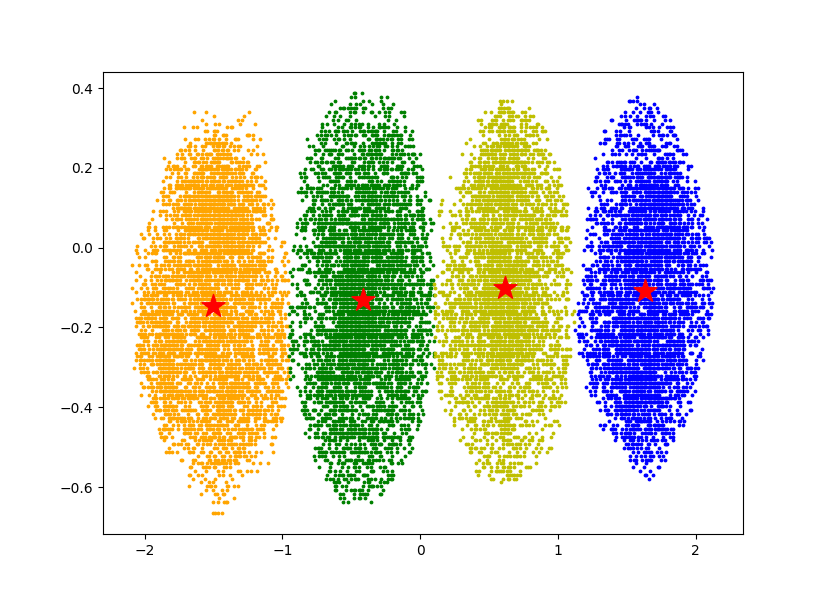
\includegraphics[width=\linewidth]{clustering_images/clustering3kmeans.png}
\centerline{Clustering 3}\\
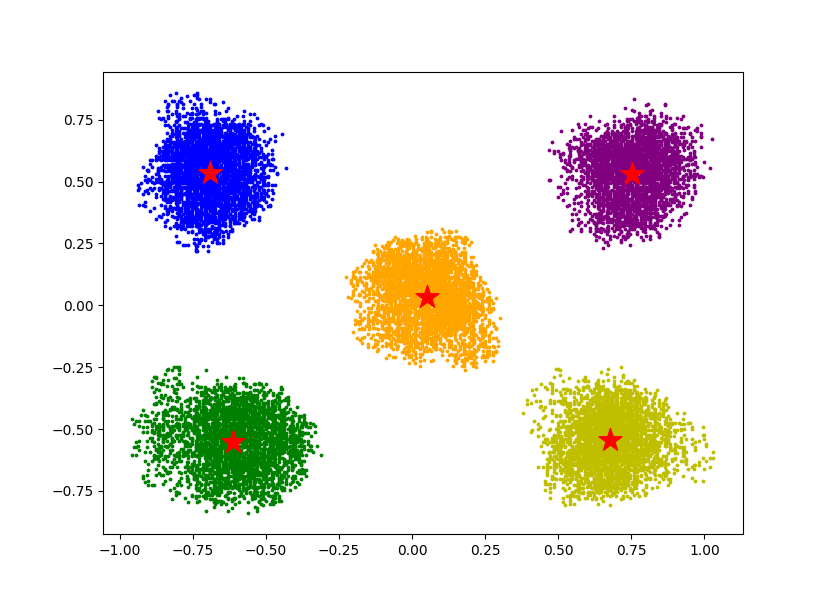
\includegraphics[width=\linewidth]{clustering_images/clustering4kmeans.png}
\centerline{Clustering 4}\\

\maketitle
\section{Part 3: Hierarchical Agglomerative Clustering}
\subsection{data1}

Since data clusters by formed by only min distances between clusters as you see single linkage performs better since inner and outer data members are more close to their inner and outer data clusters.\\

\begin{tabular}{c|c}

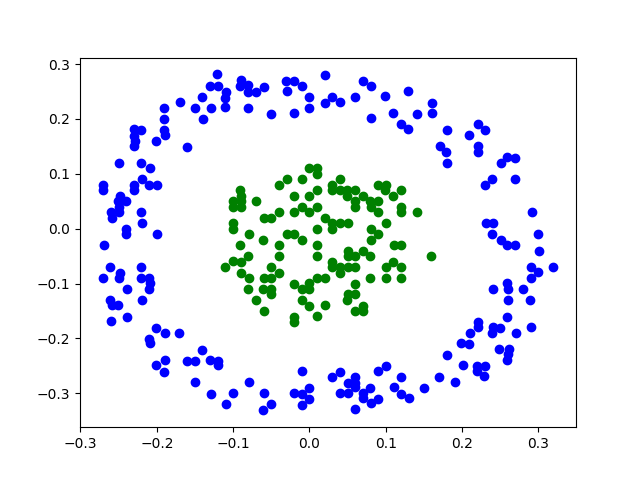
\includegraphics[scale=0.4]{hac_images/data1single.png}&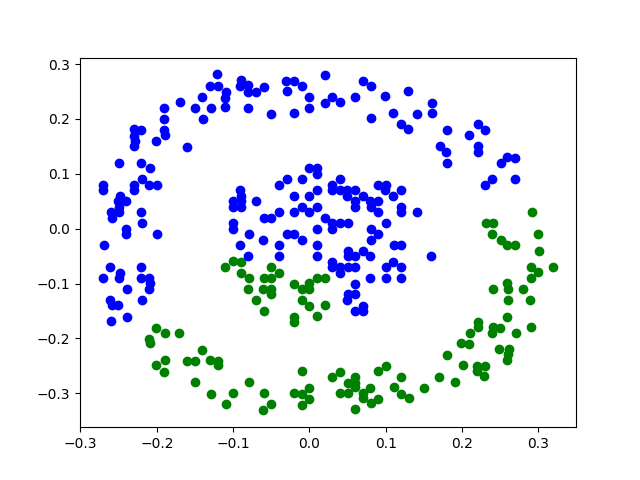
\includegraphics[scale=0.4]{hac_images/data1complete.png}\\
{Data1: Single-Linkage}&{Data1: Complete-Linkage}\\
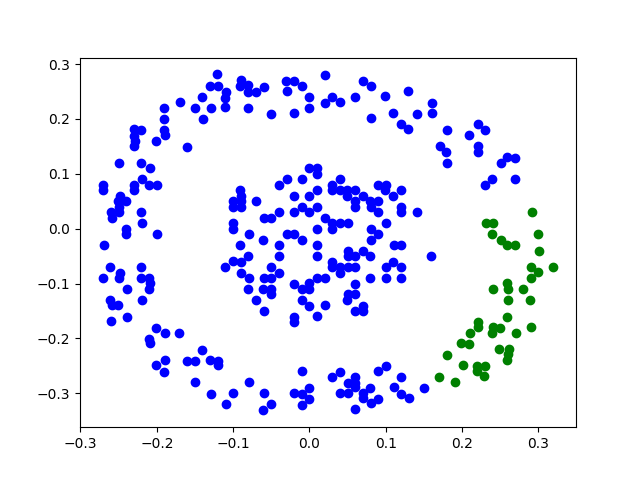
\includegraphics[scale=0.4]{hac_images/data1average.png}&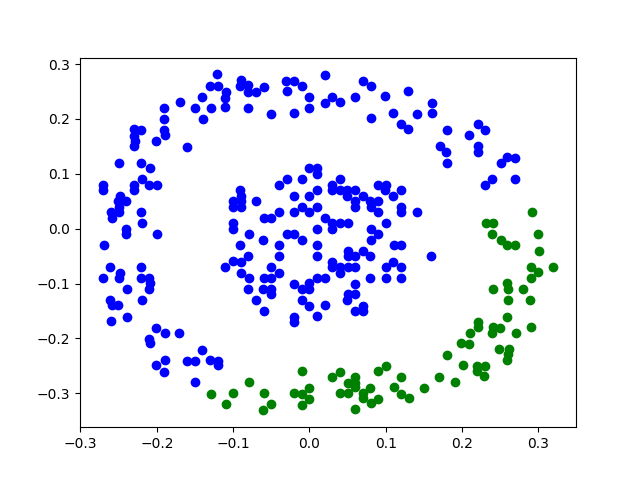
\includegraphics[scale=0.4]{hac_images/data1centroid.png}\\
{Data1: Average-Linkage}&{Data1: Centroid}\\

\end{tabular}

\subsection{data2}
Since data again has two distant clusters single linkage performs well on this data. But this time also average link performs well which will mean that clusters were merged better when their average distance
between each pair also looks like smallest distant between each cluster or so.\\
\begin{tabular}{c|c}

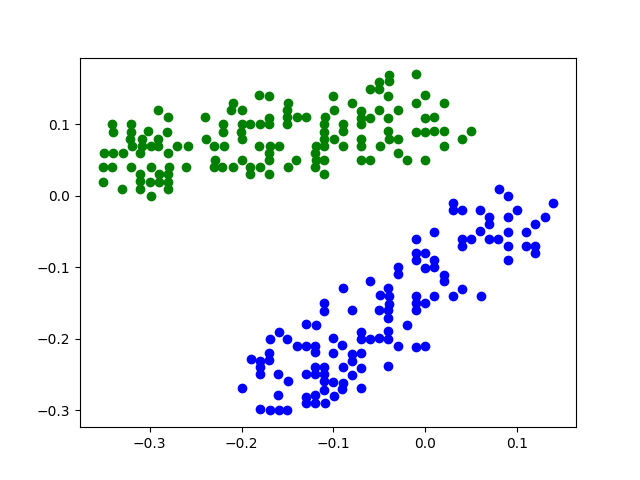
\includegraphics[scale=0.4]{hac_images/data2single.png}&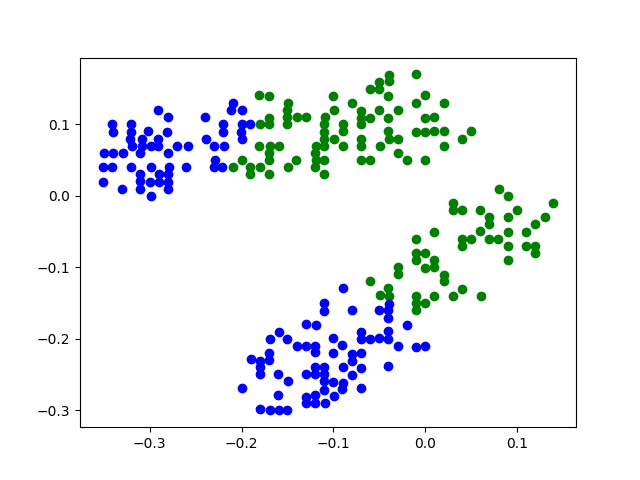
\includegraphics[scale=0.4]{hac_images/data2complete.png}\\
{Data2: Single-Linkage}&{Data2: Complete-Linkage}\\
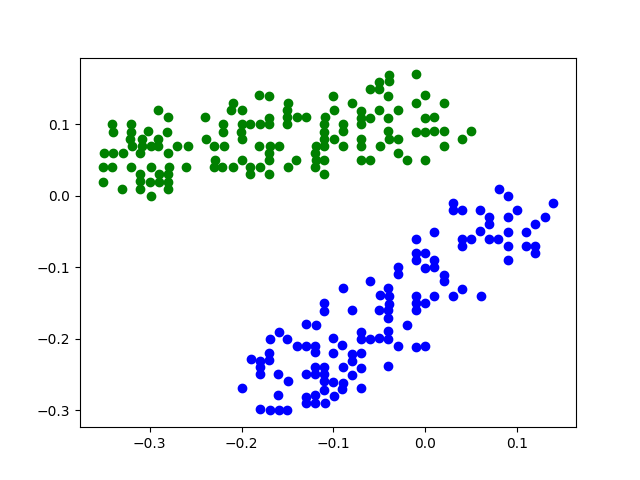
\includegraphics[scale=0.4]{hac_images/data2average.png}&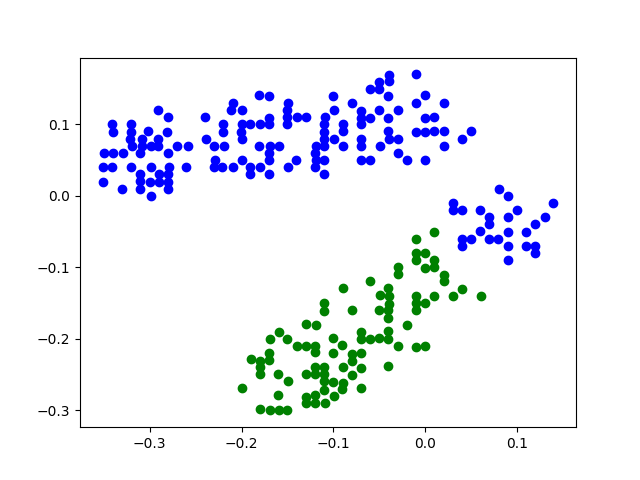
\includegraphics[scale=0.4]{hac_images/data2centroid.png}\\
{Data2: Average-Linkage}&{Data2: Centroid}\\

\end{tabular}

\subsection{data3}
Complete linkage didn't perform well on this data since cluster distances are taken as max distance between each clusters then middle side tend to join right side on our data graph as you see.\\
\begin{tabular}{c|c}

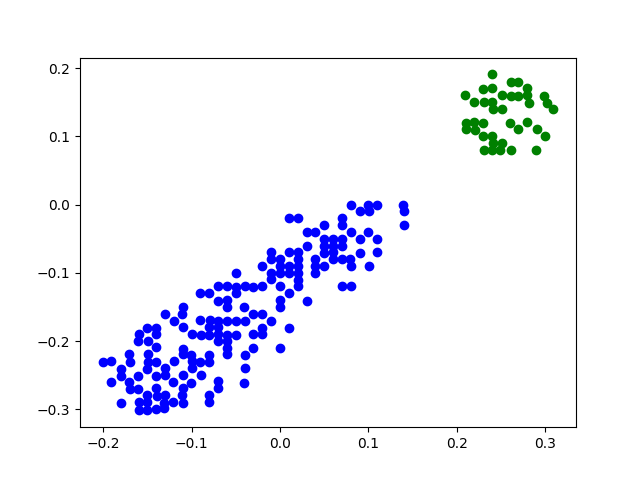
\includegraphics[scale=0.4]{hac_images/data3single.png}&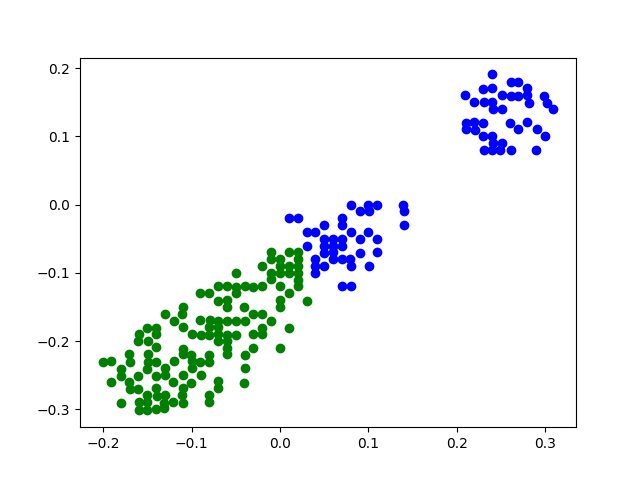
\includegraphics[scale=0.4]{hac_images/data3complete.png}\\
{Data3: Single-Linkage}&{Data3: Complete-Linkage}\\
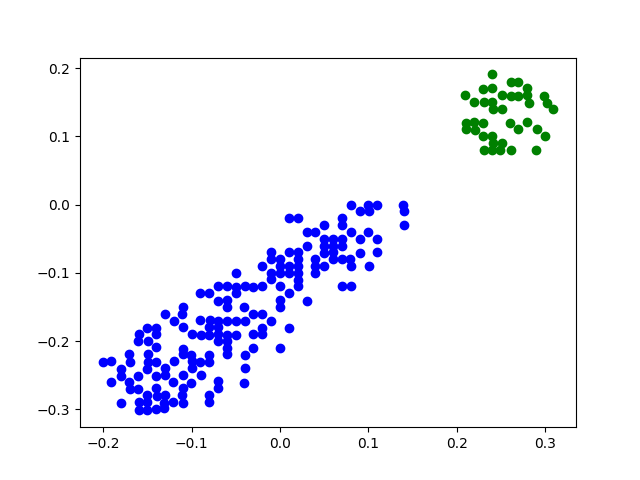
\includegraphics[scale=0.4]{hac_images/data3average.png}&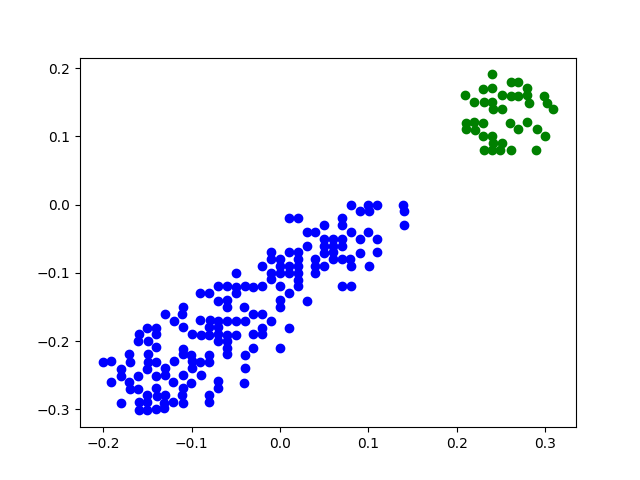
\includegraphics[scale=0.4]{hac_images/data3centroid.png}\\
{Data3: Average-Linkage}&{Data3: Centroid}\\

\end{tabular}

\subsection{data4}
Average linkage and centroid criterion fit well on this data since each cluster seems samely distributed and have same size and shape almost, they tend to join clusters in their corresponding data
places.\\

\begin{tabular}{c|c}
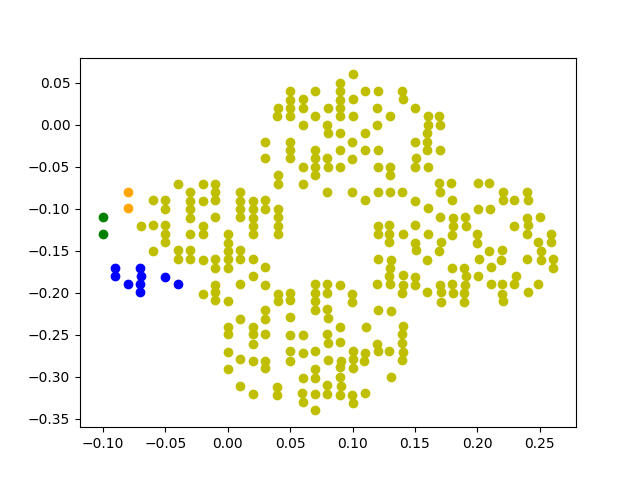
\includegraphics[scale=0.4]{hac_images/data4single.png}&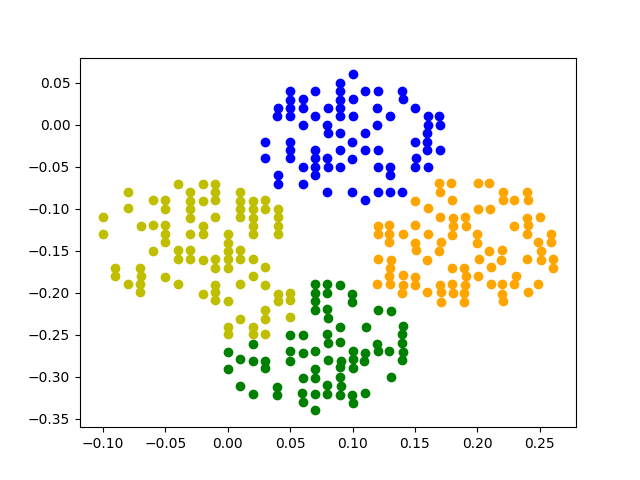
\includegraphics[scale=0.4]{hac_images/data4complete.png}\\
{Data4: Single-Linkage}&{Data4: Complete-Linkage}\\
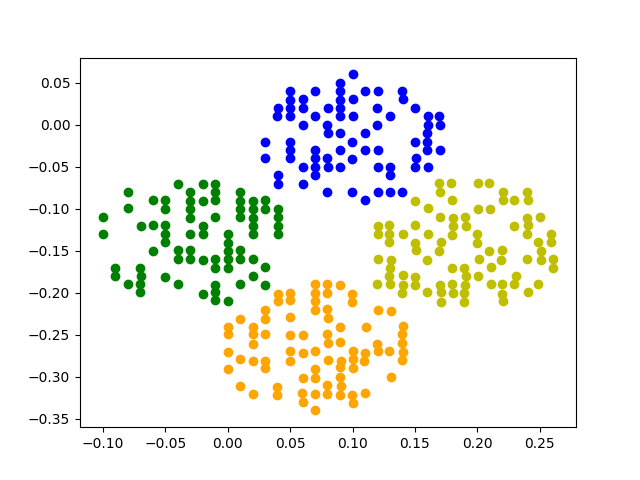
\includegraphics[scale=0.4]{hac_images/data4average.png}&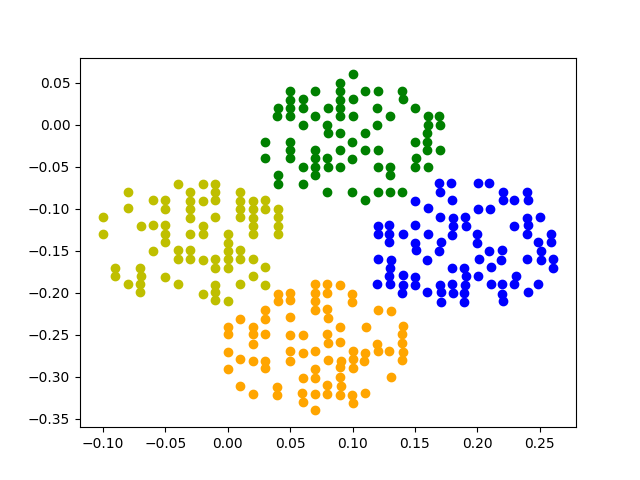
\includegraphics[scale=0.4]{hac_images/data4centroid.png}\\
{Data4: Average-Linkage}&{Data4: Centroid}\\


\end{tabular}
\end{document}

